% ============================================================
%  CS3401 – Chapter 2: Algorithm Analysis & Mathematical Background
% ============================================================
\documentclass[aspectratio=169]{beamer}
% ============================================================
%  CS3401 – Algorithm Design and Analysis
%  Shared Beamer Theme (input this file in every chapter)
%  Prince Sattam Bin Abdulaziz University – CCES
% ============================================================

% ---------- PACKAGES ----------------------------------------
\usepackage[utf8]{inputenc}
\usepackage[T1]{fontenc}
\usepackage{lmodern}
\usepackage{amsmath,amssymb,amsthm}
\usepackage{tikz}
\usepackage{pgfplots}
\usepackage{booktabs}
\usepackage{xcolor}
\usepackage{graphicx}
\usepackage{listings}
\usepackage[normalem]{ulem}
\usepackage{algorithm}
\usepackage{algpseudocode}
\usepackage{multicol}
\usepackage{array}
\usepackage{colortbl}
\usepackage{tabularx}
\usepackage{makecell}

\usetikzlibrary{
  arrows.meta, shapes.geometric, shapes.symbols,
  positioning, calc, fit, backgrounds,
  decorations.pathreplacing, decorations.markings,
  matrix, chains, trees
}
\pgfplotsset{compat=1.18}

% ---------- COLOR PALETTE -----------------------------------
\definecolor{PrimaryDark}{RGB}{10,72,92}
\definecolor{PrimaryMid}{RGB}{18,114,145}
\definecolor{PrimaryLight}{RGB}{185,224,238}
\definecolor{AccentOrange}{RGB}{210,103,22}
\definecolor{AccentYellow}{RGB}{252,198,40}
\definecolor{SuccessGreen}{RGB}{32,122,66}
\definecolor{AlertRed}{RGB}{172,46,46}
\definecolor{CodeBg}{RGB}{244,246,250}
\definecolor{DarkText}{RGB}{28,32,40}
\definecolor{LightRule}{RGB}{210,225,232}
\tikzset{processstep/.style={draw=PrimaryMid, fill=PrimaryLight!35, rounded corners=2pt,
  align=center, minimum width=4.2cm, minimum height=0.55cm, font=\small}}

% ---------- BEAMER SETTINGS ---------------------------------
\setbeamertemplate{navigation symbols}{}
\setbeamertemplate{caption}[numbered]

% Fonts
\setbeamerfont{normal text}{size=\small}
\setbeamerfont{title}{series=\bfseries,size=\LARGE}
\setbeamerfont{subtitle}{series=\normalfont,size=\large}
\setbeamerfont{frametitle}{series=\bfseries,size=\large}
\setbeamerfont{framesubtitle}{series=\normalfont,size=\small}
\setbeamerfont{block title}{series=\bfseries,size=\normalsize}
\setbeamerfont{footline}{size=\tiny}
\addtobeamertemplate{frame begin}{\small\enlargethispage{1cm}}{}
\setlength{\tabcolsep}{2pt}

% Colors
\setbeamercolor{normal text}{fg=DarkText,bg=white}
\setbeamercolor{frametitle}{bg=PrimaryDark,fg=white}
\setbeamercolor{title}{fg=white}
\setbeamercolor{subtitle}{fg=PrimaryLight}
\setbeamercolor{author}{fg=white}
\setbeamercolor{date}{fg=PrimaryLight}
\setbeamercolor{institute}{fg=PrimaryLight}
\setbeamercolor{block title}{bg=PrimaryMid,fg=white}
\setbeamercolor{block body}{bg=PrimaryLight!35,fg=DarkText}
\setbeamercolor{block title alerted}{bg=AlertRed,fg=white}
\setbeamercolor{block body alerted}{bg=AlertRed!12,fg=DarkText}
\setbeamercolor{block title example}{bg=SuccessGreen,fg=white}
\setbeamercolor{block body example}{bg=SuccessGreen!12,fg=DarkText}
\setbeamercolor{itemize item}{fg=PrimaryMid}
\setbeamercolor{itemize subitem}{fg=AccentOrange}
\setbeamercolor{enumerate item}{fg=PrimaryMid}
\setbeamercolor{enumerate subitem}{fg=AccentOrange}
\setbeamercolor{alerted text}{fg=AlertRed}
\setbeamercolor{structure}{fg=PrimaryMid}
\setbeamercolor{section in toc}{fg=PrimaryDark}
\setbeamercolor{section in toc shaded}{fg=PrimaryDark}
% override Beamer's transparency-based shading so TOC entries stay fully visible
\setbeamertemplate{section in toc shaded}{\inserttocsection\par}
\setbeamercolor{subsection in toc}{fg=PrimaryMid}
\setbeamercolor{footer rule}{bg=LightRule}

% Item symbols
\setbeamertemplate{itemize item}{%
  \scriptsize\raise1.5pt\hbox{\color{PrimaryMid}$\blacktriangleright$}}
\setbeamertemplate{itemize subitem}{%
  \scriptsize\raise1pt\hbox{\color{AccentOrange}$\bullet$}}
\setbeamertemplate{itemize subsubitem}{%
  \scriptsize\raise1pt\hbox{\color{PrimaryDark}$\circ$}}
\setbeamertemplate{enumerate item}{%
  \color{PrimaryMid}\textbf{\insertenumlabel.}}

% Frame title
\makeatletter
\setbeamertemplate{frametitle}{%
  \nointerlineskip
  \begin{beamercolorbox}[wd=\paperwidth,ht=2.4em,dp=0.9em,%
                         leftskip=1.2em,rightskip=1.2em]{frametitle}
    \usebeamerfont{frametitle}\insertframetitle\strut
    \ifx\insertframesubtitle\@empty\else
      \hspace{0.6em}\textcolor{PrimaryLight!80}{\footnotesize|}\hspace{0.4em}%
      {\usebeamerfont{framesubtitle}\textcolor{PrimaryLight}\insertframesubtitle}%
    \fi
  \end{beamercolorbox}
  \nointerlineskip
  \begin{beamercolorbox}[wd=\paperwidth,ht=0.3pt,dp=0pt]{structure}
  \end{beamercolorbox}
}
\makeatother

% Footer
\setbeamertemplate{footline}{%
  \begin{beamercolorbox}[wd=\paperwidth,ht=0.4pt,dp=0pt]{footer rule}{}
  \end{beamercolorbox}
  \leavevmode
  \hbox{%
    \begin{beamercolorbox}[wd=0.60\paperwidth,ht=1.8em,dp=0.6em,leftskip=1em]{normal text}%
      \textcolor{PrimaryDark}{\tiny\textbf{CS3401} \textendash{} Algorithm Design \& Analysis%
        \quad\textbar\quad CCES, PSAU}%
    \end{beamercolorbox}%
    \begin{beamercolorbox}[wd=0.40\paperwidth,ht=1.8em,dp=0.6em,rightskip=1em,right]{normal text}%
      \textcolor{PrimaryDark}{\tiny\insertshorttitle%
        \quad\textbar\quad\insertframenumber\,/\,\inserttotalframenumber}%
    \end{beamercolorbox}%
  }%
}

% Title page
\setbeamertemplate{title page}{%
  
\begin{tikzpicture}[remember picture,overlay]
    \fill[PrimaryDark](current page.north west) rectangle (current page.south east);
    \fill[PrimaryMid,opacity=0.45]
      ([shift={(2.5cm,-2.5cm)}]current page.north east) circle(5.5cm);
    \fill[AccentOrange,opacity=0.10]
      ([shift={(-1.5cm,2.0cm)}]current page.south west) circle(4.2cm);
    \draw[white,opacity=0.08,line width=40pt]
      ([shift={(0cm,-0.5cm)}]current page.north west)
      to[out=-30,in=210]
      ([shift={(0cm,0.5cm)}]current page.south east);
  \end{tikzpicture}%
  \vspace{0.7cm}
  \begin{center}
    {\tiny\textcolor{PrimaryLight}{\textbf{CCES} \textendash{}
      College of Computer Engineering and Sciences}}\\[0.2em]
    {\tiny\textcolor{PrimaryLight}{Prince Sattam Bin Abdulaziz University}}\\[1.2em]
    {\footnotesize\textcolor{AccentYellow}{\textbf{CS3401 \textendash{} Algorithm Design and Analysis}}}\\[1.5em]
    \textcolor{PrimaryMid}{\rule{0.55\textwidth}{0.6pt}}\\[0.9em]
    {\Large\usebeamerfont{title}\textcolor{white}{\inserttitle}}\\[0.4em]
    {\small\usebeamerfont{subtitle}\textcolor{PrimaryLight}{\insertsubtitle}}\\[0.7em]
    \textcolor{PrimaryMid}{\rule{0.55\textwidth}{0.6pt}}\\[1.2em]
    {\footnotesize\textcolor{PrimaryLight}{\insertdate}}\\[0.6em]
    % Instructors row
    \begin{tikzpicture}[baseline=(current bounding box.center)]
      % Dr. Khalil – rounded photo
      \begin{scope}
        \clip (-3.2,0) circle (0.58cm);
        \node at (-3.2,0)
          {
\includegraphics[width=1.16cm,height=1.16cm,keepaspectratio=false]{khalil}};
      \end{scope}
      \draw[white,line width=0.9pt] (-3.2,0) circle (0.58cm);
      \node[text=white,font=\scriptsize\bfseries,anchor=west] at (-2.54,0)
        {Dr.\ Khalil Chebil};
      % Dr. Esraa – placeholder circle
      \draw[white,line width=0.9pt] (1.2,0) circle (0.58cm);
      \node[text=PrimaryLight,font=\normalsize\bfseries] at (1.2,0) {E};
      \node[text=white,font=\scriptsize\bfseries,anchor=west] at (1.86,0)
        {Dr.\ Esraa};
    \end{tikzpicture}
  \end{center}%
}

% Auto section-divider slide — background set via Beamer color system for reliability
\AtBeginSection[]{%
  {%
    \setbeamercolor{background canvas}{bg=PrimaryDark}%
    \begin{frame}[plain,noframenumbering]
      \begin{tikzpicture}[remember picture,overlay]
        \fill[PrimaryMid,opacity=0.35]
          ([shift={(0cm,-1.5cm)}]current page.north) circle(6.5cm);
        \node[text=white,opacity=0.06,font=\fontsize{120}{120}\bfseries]
          at ([shift={(-1cm,0cm)}]current page.center)
          {\insertsectionnumber};
      \end{tikzpicture}
      \vfill
      \begin{center}
        {\large\textcolor{AccentYellow}{\textbf{Section \insertsectionnumber}}}\\[0.6em]
        {\LARGE\textcolor{white}{\textbf{\insertsectionhead}}}
      \end{center}
      \vfill
    \end{frame}
  }%
}

% ---------- LISTINGS STYLE ----------------------------------
\lstset{
  basicstyle=\ttfamily\footnotesize,
  backgroundcolor=\color{CodeBg},
  keywordstyle=\color{PrimaryMid}\bfseries,
  commentstyle=\color{SuccessGreen}\itshape,
  stringstyle=\color{AccentOrange},
  numberstyle=\tiny\color{gray!70},
  frame=tb,
  framerule=0.5pt,
  rulecolor=\color{PrimaryLight},
  numbers=left,
  numbersep=6pt,
  showstringspaces=false,
  breaklines=true,
  tabsize=2,
  xleftmargin=1.8em,
  framexleftmargin=1.8em,
  captionpos=b,
  language=Java,
  morekeywords={var,let,const}
}

% ---------- PSEUDOCODE STYLE --------------------------------
\algrenewcommand\algorithmicprocedure{\textbf{Algorithm}}
\algrenewcommand\algorithmicfunction{\textbf{Function}}
\algrenewcommand\algorithmicif{\textbf{if}}
\algrenewcommand\algorithmicelse{\textbf{else}}
\algrenewcommand\algorithmicthen{\textbf{then}}
\algrenewcommand\algorithmicwhile{\textbf{while}}
\algrenewcommand\algorithmicfor{\textbf{for}}
\algrenewcommand\algorithmicforall{\textbf{for all}}
\algrenewcommand\algorithmicreturn{\textbf{return}}
\algrenewcommand\algorithmicend{\textbf{end}}
\algrenewcommand\algorithmicdo{}
\algrenewcommand\algorithmicrequire{\textbf{Input:}}
\algrenewcommand\algorithmicensure{\textbf{Output:}}

% ---------- CUSTOM COMMANDS ---------------------------------
\newcommand{\bigO}[1]{$\mathcal{O}(#1)$}
\newcommand{\bigTheta}[1]{$\Theta(#1)$}
\newcommand{\bigOmega}[1]{$\Omega(#1)$}
\newcommand{\highlight}[1]{\colorbox{AccentYellow!55}{\strut #1}}
\newcommand{\important}[1]{\textcolor{AlertRed}{\bfseries #1}}
\newcommand{\keyword}[1]{\textcolor{PrimaryMid}{\bfseries #1}}
\newcommand{\concept}[1]{\textcolor{AccentOrange}{\bfseries #1}}

% Colored table column types
\newcolumntype{H}{>{\columncolor{PrimaryDark}\color{white}\bfseries\centering\arraybackslash}m{2.5cm}}
\newcolumntype{Z}{>{\columncolor{PrimaryLight!40}\centering\arraybackslash}m{2cm}}

% Reference boxes
\newcommand{\refbox}[1]{%
  \begin{beamercolorbox}[rounded=true,shadow=false,leftskip=0.5em,rightskip=0.5em,%
                          ht=1.6em,dp=0.5em]{block title}
    \small\textit{Reference:} #1
  \end{beamercolorbox}%
}

% Inline complexity tag
\newcommand{\ctag}[1]{%
  \hfill\tikz[baseline]{\node[fill=AlertRed,text=white,rounded corners=2pt,
    font=\bfseries\scriptsize,inner sep=2pt,outer sep=0pt]{$\mathcal{O}(#1)$};}%
}


\title[Ch.\,2 -- Algorithm Analysis]{Chapter 2}
\subtitle{Algorithm Analysis \& Mathematical Background}
\date{Academic Year 2026\,--\,2027}

\begin{document}

\begin{frame}[plain]\titlepage\end{frame}

\begin{frame}{Chapter Overview}
  \begin{center}
    \begin{minipage}{0.85\textwidth}
      \tableofcontents[hideallsubsections,sectionstyle=show/shaded]
    \end{minipage}
  \end{center}
\end{frame}

% ============================================================
\section{Theoretical Analysis of Time Efficiency}
% ============================================================

\begin{frame}[shrink=12]{Objectives}
  After this chapter you will be able to:
  \begin{itemize}
    \item Estimate the running time of an algorithm \emph{without} running it
        \item Apply \textbf{Big-O}, \textbf{Big-Omega}, and
          \textbf{Big-Theta} notation correctly
    \item Use the \emph{limit method} to compare growth rates
    \item Identify worst-case, best-case, and average-case complexities
    \item Apply the \emph{Master Theorem} to divide-and-conquer recurrences
    \item Analyse iterative and recursive algorithms systematically
  \end{itemize}
  \vspace{0.4em}
  \begin{block}{Why does this matter?}
    Before writing a single line of code, analysis tells you whether your
    algorithm will finish in milliseconds — or centuries.
  \end{block}
\end{frame}

\begin{frame}[shrink=12]{Theoretical Framework}
  \begin{block}{Running Time Model}
    \[
      T(n) \;\approx\; c_{\mathrm{op}} \cdot C(n)
    \]
    \begin{center}
      \small
      $c_{\mathrm{op}}$ = execution time of one basic operation \quad
      $C(n)$ = \# times the basic operation executes on input of size $n$
    \end{center}
  \end{block}
  \vspace{0.4em}
  \begin{columns}[T]
    \column{0.48\textwidth}
      \textbf{Input size measure examples:}
      \vspace{0.2em}

      \begin{tabular}{ll}
        \toprule
        \textbf{Problem} & \textbf{Input size} \\
        \midrule
        Searching in a list & $n$ = list length \\
        Matrix multiplication & $n\times n$ dimension \\
        Primality test & \# bits of $n$ \\
        Graph traversal & $|V| + |E|$ \\
        \bottomrule
      \end{tabular}
    \column{0.48\textwidth}
      \textbf{Basic operation examples:}
      \vspace{0.2em}

      \begin{tabular}{ll}
        \toprule
        \textbf{Problem} & \textbf{Basic op.} \\
        \midrule
        Searching & key comparison \\
        Sorting & element comparison \\
        Matrix multiply & multiplication \\
        Polynomial eval. & multiplication \\
        \bottomrule
      \end{tabular}
  \end{columns}
\end{frame}

\begin{frame}[shrink=12]{Worst, Best, and Average Case}
  \begin{columns}[T]
    \column{0.55\textwidth}
      \begin{block}{Three complexity measures}
        \begin{itemize}
          \item $C_{\text{worst}}(n)$ — maximum over all inputs of size $n$\\
                \textit{Provides an upper bound guarantee}
          \item $C_{\text{best}}(n)$ — minimum over all inputs of size $n$\\
                \textit{Often unrealistically optimistic}
          \item $C_{\text{avg}}(n)$ — \emph{expected} count assuming a
                probability distribution over inputs\\
                \textit{Harder to compute; most realistic}
        \end{itemize}
      \end{block}
      \vspace{0.3em}
      \begin{alertblock}{Important note}
        $C_{\text{avg}}(n)$ is \important{not} the average of worst and best
        case — it is a probabilistic expectation.
      \end{alertblock}
    \column{0.40\textwidth}
      \textbf{Example: Sequential Search}
      \begin{algorithmic}[1]
        \Require Array $A[0..n{-}1]$, key $K$
        \State $i \gets 0$
        \While{$i < n$ \textbf{and} $A[i] \neq K$}
          \State $i \gets i + 1$
        \EndWhile
        \If{$i < n$} \Return $i$
        \Else\; \Return $-1$
        \EndIf
      \end{algorithmic}
      \vspace{0.3em}
      \begin{tabular}{ll}
        Best:    & 1 comparison \\
        Worst:   & $n$ comparisons \\
        Average: & $\dfrac{n+1}{2}$ comparisons \\
      \end{tabular}
  \end{columns}
\end{frame}

% ============================================================
\section{Asymptotic Notation}
% ============================================================

\begin{frame}[shrink=20]{Big-O Notation — Upper Bound}
  \begin{block}{Definition}
    $T(n) = \mathcal{O}(f(n))$ if there exist positive constants $c$ and $n_0$
    such that
    \[
      T(n) \;\leq\; c\,f(n) \quad \text{for all } n \geq n_0
    \]
  \end{block}
  \vspace{0.3em}
  \begin{columns}[T]
    \column{0.50\textwidth}
      \textbf{Intuition:} $T(n) = \mathcal{O}(f(n))$ means $T$ grows
      \emph{no faster than} $f$.
      \vspace{0.4em}

      \textbf{Examples:}
      \begin{itemize}
        \item $3n^2 + 2n = \mathcal{O}(n^2)$
        \item $100\log n = \mathcal{O}(\log n)$
        \item $2^n + n^{100} = \mathcal{O}(2^n)$
      \end{itemize}
      \vspace{0.4em}
      \begin{alertblock}{Common mistakes}
        \textit{Do not} write $\mathcal{O}(2n^2)$ or $\mathcal{O}(n^2+n)$.
        Drop constants and lower-order terms.
        The correct form is $\mathcal{O}(n^2)$.
      \end{alertblock}
    \column{0.45\textwidth}
      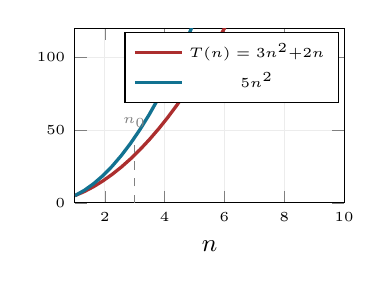
\begin{tikzpicture}
        \begin{axis}[
          width=5.0cm,height=3.8cm,
          xlabel={\small $n$},ylabel={},
          xmin=1,xmax=10,ymin=0,ymax=120,
          tick label style={font=\tiny},
          label style={font=\small},
          grid=major,grid style={gray!15},
          no markers,
          legend style={font=\tiny,at={(0.98,0.98)},anchor=north east}
        ]
          \addplot[AlertRed,very thick,domain=1:10,samples=30]{3*x^2+2*x};
          \addplot[PrimaryMid,very thick,domain=1:10,samples=30]{5*x^2};
          \draw[gray,dashed] (axis cs:3,0) -- (axis cs:3,45)
            node[above,font=\tiny]{$n_0$};
          \legend{$T(n)=3n^2{+}2n$,$5n^2$}
        \end{axis}
      \end{tikzpicture}
  \end{columns}
\end{frame}

\begin{frame}[shrink=20]{Big-$\Omega$ and Big-$\Theta$ Notation}
  \begin{columns}[T]
    \column{0.48\textwidth}
      \begin{block}{Big-$\Omega$ — Lower Bound}
        $T(n) = \Omega(g(n))$ if $\exists\,c, n_0 > 0$ such that
        \[
          T(n) \;\geq\; c\,g(n) \quad \forall\, n \geq n_0
        \]
        \textit{Intuition:} $T$ grows \emph{at least as fast} as $g$.\\[0.3em]
        \textit{Example:} $n^4 = \Omega(n^3)$
      \end{block}
      \vspace{0.4em}
      \begin{block}{Big-$\Theta$ — Tight Bound}
        $T(n) = \Theta(h(n))$ iff
        $T(n) = \mathcal{O}(h(n))$ \textbf{and} $T(n) = \Omega(h(n))$
        \vspace{0.2em}

        \textit{Intuition:} $T$ and $h$ grow at the \emph{same rate}.\\[0.3em]
        \textit{Key fact:} If $T(n)$ is a degree-$k$ polynomial,
        then $T(n) = \Theta(n^k)$.\\[0.3em]
        \textit{Example:} $2n^4 = \Theta(n^4)$
      \end{block}
    \column{0.48\textwidth}
      \begin{block}{Little-o and Little-$\omega$}
        $T(n) = o(f(n))$: $T$ grows \emph{strictly slower} than $f$\\
        \quad ($T(n)=\mathcal{O}(f(n))$ but $T(n)\neq\Theta(f(n))$)\\[0.3em]
        $T(n) = \omega(f(n))$: $T$ grows \emph{strictly faster} than $f$
      \end{block}
      \vspace{0.4em}
      \begin{block}{Composition rules}
        If $T_1 = \mathcal{O}(f)$ and $T_2 = \mathcal{O}(g)$, then:
        \begin{itemize}
          \item $T_1 + T_2 = \mathcal{O}(\max(f,g))$
          \item $T_1 \cdot T_2 = \mathcal{O}(f\cdot g)$
        \end{itemize}
        \textit{Example:} $\mathcal{O}(n^2)+\mathcal{O}(n)=\mathcal{O}(n^2)$
      \end{block}
  \end{columns}
\end{frame}

\begin{frame}[shrink=12]{Typical Growth Rates}
  \begin{columns}[T]
    \column{0.38\textwidth}
      \begin{tabular}{ll}
        \toprule
        \textbf{Function} & \textbf{Name} \\
        \midrule
        $c$ & Constant \\
        $\log n$ & Logarithmic \\
        $\log^2 n$ & Log-squared \\
        $n$ & Linear \\
        $n\log n$ & Linearithmic \\
        $n^2$ & Quadratic \\
        $n^3$ & Cubic \\
        $2^n$ & Exponential \\
        $n!$ & Factorial \\
        \bottomrule
      \end{tabular}
      \newline
      \vspace{0.3em}
      \small (Ordered by increasing growth rate)
    \column{0.58\textwidth}
      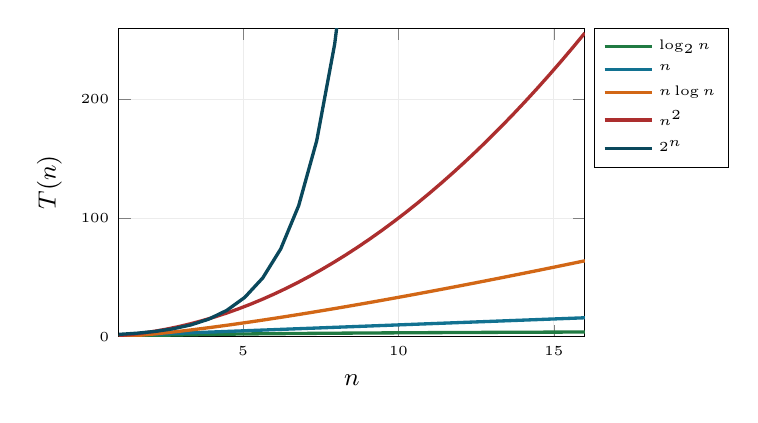
\begin{tikzpicture}
        \begin{axis}[
          width=7.5cm, height=5.5cm,
          xlabel={\small $n$}, ylabel={\small $T(n)$},
          xmin=1, xmax=16, ymin=0, ymax=260,
          tick label style={font=\tiny},
          label style={font=\small},
          grid=major, grid style={gray!15},
          no markers,
          legend style={font=\tiny,at={(1.02,1)},anchor=north west,
                        cells={anchor=west}}
        ]
          \addplot[SuccessGreen,very thick,domain=1:16,samples=40]{ln(x)/ln(2)};
          \addplot[PrimaryMid,very thick,domain=1:16,samples=40]{x};
          \addplot[AccentOrange,very thick,domain=1:16,samples=40]{x*ln(x)/ln(2)};
          \addplot[AlertRed,very thick,domain=1:16,samples=40]{x^2};
          \addplot[PrimaryDark,very thick,domain=1:12,samples=20]{2^x};
          \legend{$\log_2 n$, $n$, $n\log n$, $n^2$, $2^n$}
        \end{axis}
      \end{tikzpicture}
  \end{columns}
\end{frame}

\begin{frame}[shrink=12]{Establishing Order of Growth: The Limit Method}
  \[
    \lim_{n\to\infty}\frac{T(n)}{g(n)} =
    \begin{cases}
      0       & \Rightarrow T(n) = o(g(n)) \quad\text{(T grows slower)} \\
      c > 0   & \Rightarrow T(n) = \Theta(g(n)) \quad\text{(same rate)} \\
      \infty  & \Rightarrow T(n) = \omega(g(n)) \quad\text{(T grows faster)}
    \end{cases}
  \]
  \vspace{0.3em}
  \begin{columns}[T]
    \column{0.50\textwidth}
      \textbf{Example 1:} Compare $10n$ vs $n^2$
      \[
        \lim_{n\to\infty}\frac{10n}{n^2} = \lim_{n\to\infty}\frac{10}{n} = 0
        \implies 10n = o(n^2)
      \]
    \column{0.46\textwidth}
      \textbf{Example 2:} Compare $\dfrac{n(n-1)}{2}$ vs $n^2$
      \[
        \lim_{n\to\infty}\frac{n(n-1)/2}{n^2}
        = \frac{1}{2}\lim_{n\to\infty}\!\left(1 - \frac{1}{n}\right)
        = \frac{1}{2}
      \]
      $\implies \dfrac{n(n-1)}{2} = \Theta(n^2)$
  \end{columns}
  \vspace{0.4em}
  \begin{exampleblock}{Practice}
    Use the limit method to show: $n^3 = o(n^4)$ and $5n^2+3n = \Theta(n^2)$
  \end{exampleblock}
\end{frame}

\begin{frame}[shrink=28]{Case Study: Leaderboard Ranking}
  \begin{block}{Problem}
    A gaming platform stores $n$ player scores. After each match, find the
    \emph{top-$k$} players and check whether a given player is in the top-$k$.
  \end{block}
  \vspace{0.3em}
  \begin{columns}[T]
    \column{0.52\textwidth}
      \textbf{Three approaches:}
      \vspace{0.2em}

      \begin{tabular}{@{}lll@{}}
        \toprule
        \textbf{Algorithm} & \textbf{Preprocessing} & \textbf{Per query} \\
        \midrule
        Linear scan       & none              & $\mathcal{O}(n)$ \\
        Sort once         & $\Theta(n\log n)$ & $\mathcal{O}(1)$ \\
        Max-heap (top-$k$)& $\Theta(n\log k)$ & $\mathcal{O}(\log k)$ \\
        \bottomrule
      \end{tabular}
      \vspace{0.4em}

      \textbf{Classifying the sort cost} $T(n) = 5n\log_2 n + 3n + 7$:
      \[
        \lim_{n\to\infty}\frac{5n\log_2 n + 3n + 7}{n\log n}
        = 5 \implies \Theta(n\log n)
      \]
      Lower-order terms $3n$ and constant $7$ are \emph{absorbed}.

    \column{0.44\textwidth}
      \textbf{Scaling to 10 million players:}
      \vspace{0.2em}
      \begin{tabular}{@{}lrr@{}}
        \toprule
        & $n{=}10^4$ & $n{=}10^6$ \\
        \midrule
        Linear / query  & 0.1 ms   & 10 ms \\
        After sort      & 0.000 ms & 0.000 ms \\
        \bottomrule
      \end{tabular}
      \vspace{0.4em}
      \begin{exampleblock}{Lesson}
        Asymptotic notation ignores constants and lower-order terms —
        what matters is the \emph{dominant term}:
        \begin{itemize}
          \item $5n\log n + 3n + 7 = \Theta(n\log n)$
          \item $7 = \Theta(1)$ (constant $\not\Rightarrow$ free)
          \item $n^2 + 10^6 n = \Theta(n^2)$
        \end{itemize}
      \end{exampleblock}
  \end{columns}
\end{frame}

% ============================================================
\section{Running Time Calculation}
% ============================================================

\begin{frame}[fragile,shrink=12]{Calculating Running Time — A Simple Example}
  \begin{columns}[T]
    \column{0.45\textwidth}
      \begin{lstlisting}[language=Java,numbers=left]
int sum(int n) {             // 1 op
  int i, partialSum;         // 0 ops (declarations)
  partialSum = 0;            // 1 op
  for (i = 1; i <= n; i++)  // 1+n+1+n = 2N+2
    partialSum += i*i*i;     // 4 ops * N = 4N
  return partialSum;         // 1 op
}
      \end{lstlisting}
    \column{0.50\textwidth}
      \textbf{Operation count:}
      \begin{itemize}
        \item Initialization: $1$ (partialSum)
        \item Loop setup: $1$ (i=1), $N+1$ tests, $N$ increments $= 2N+2$
        \item Loop body: $4N$ (two multiplications, one addition, one assignment)
        \item Return: $0$ (ignored)
      \end{itemize}
      \[
        \text{Total} = 1 + 2N + 2 + 4N + 1 = 6N + 4
      \]
      \[
        \implies T(n) = \mathcal{O}(N)
      \]
  \end{columns}
\end{frame}

\begin{frame}[shrink=20]{General Rules for Running Time}
  \begin{columns}[T]
    \column{0.48\textwidth}
      \begin{block}{Rule 1 — For loop}
        $T_{\text{loop}} = $ (loop body cost) $\times$ (\# iterations)
        \vspace{0.2em}

        \texttt{for (i=1; i<=n; i++) k++;}\quad$\to\mathcal{O}(n)$
      \end{block}
      \vspace{0.3em}
      \begin{block}{Rule 2 — Nested loops}
        Multiply the costs of all loops.
        \vspace{0.2em}

        \begin{algorithmic}[1]
          \For{$i \gets 0$ to $n{-}1$}
            \For{$j \gets 0$ to $n{-}1$}
              \State $k\mathrel{+}= 1$
            \EndFor
          \EndFor
        \end{algorithmic}
        $\to\mathcal{O}(n^2)$
      \end{block}
    \column{0.48\textwidth}
      \begin{block}{Rule 3 — Consecutive statements}
        Take the maximum (the dominant term).
        \vspace{0.2em}

        $\mathcal{O}(n) + \mathcal{O}(n^2) = \mathcal{O}(n^2)$
      \end{block}
      \vspace{0.3em}
      \begin{block}{Rule 4 — Conditional}
        The running time of \texttt{if-else} is bounded by
        the \emph{larger} of the two branches.
        \vspace{0.2em}

        $\max(\mathcal{O}(S_1),\; \mathcal{O}(S_2))$
      \end{block}
      \vspace{0.3em}
      \begin{alertblock}{Two useful identities}
        $\displaystyle\sum_{i=1}^{N} i = \frac{N(N+1)}{2} \in \Theta(N^2)$\\[4pt]
        $\displaystyle\sum_{i=1}^{N} i^2 = \frac{N(2N+1)(N+1)}{6} \in \Theta(N^3)$
      \end{alertblock}
  \end{columns}
\end{frame}

\begin{frame}[shrink=12]{Loop Analysis: Two Worked Examples}
  \begin{columns}[T]
    \column{0.48\textwidth}
      \textbf{Example A — $\mathcal{O}(N^2)$}
      \begin{algorithmic}[1]
        \State $\text{sum} \gets 0$
        \For{$j \gets 0$ to $n{-}1$}
          \For{$k \gets 0$ to $j{-}1$}
            \State $\text{sum}\mathrel{+}= 1$
          \EndFor
        \EndFor
      \end{algorithmic}
      \vspace{0.3em}
      \[
        \sum_{j=0}^{N-1}\sum_{k=0}^{j-1}1
        = \sum_{j=0}^{N-1}j
        = \frac{(N-1)N}{2} \in \Theta(N^2)
      \]
    \column{0.48\textwidth}
      \textbf{Example B — $\mathcal{O}(N^3)$}
      \begin{algorithmic}[1]
        \State $\text{sum} \gets 0$
        \For{$j \gets 0$ to $n{-}1$}
          \For{$k \gets 0$ to $n^2{-}1$}
            \State $\text{sum}\mathrel{+}= 1$
          \EndFor
        \EndFor
      \end{algorithmic}
      \vspace{0.3em}
      \[
        \sum_{j=0}^{N-1}\sum_{k=0}^{N^2-1}1
        = \sum_{j=0}^{N-1}N^2 = N^3 \in \Theta(N^3)
      \]
  \end{columns}
  \vspace{0.3em}
  \begin{alertblock}{Key point}
    Always simplify the inner sum \emph{before} multiplying. Look at the
    upper limit of $k$ carefully — it may depend on $j$ or on $n$.
  \end{alertblock}
\end{frame}

% ============================================================
\section{Logarithms in Running Time}
% ============================================================

\begin{frame}[shrink=12]{$\mathcal{O}(\log n)$ Algorithms}
  \begin{block}{When does $\log n$ appear?}
    An algorithm runs in $\mathcal{O}(\log n)$ if it \emph{halves}
    the problem size at each step in $\mathcal{O}(1)$ work.
  \end{block}
  \vspace{0.3em}
  \begin{columns}[T]
    \column{0.50\textwidth}
      \textbf{Fast Exponentiation: $X^N$}
      \[
        X^N = \begin{cases}
          1                       & N = 0 \\
          X                       & N = 1 \\
          (X^{N/2})^2             & N \text{ even} \\
          (X^{(N-1)/2})^2 \cdot X & N \text{ odd}
        \end{cases}
      \]
      \vspace{0.2em}
      Recurrence: $T(N) = T(N/2) + c \implies T(N) = \mathcal{O}(\log N)$
    \column{0.45\textwidth}
      \textbf{Derivation of $\mathcal{O}(\log N)$:}
      \begin{align*}
        T(N) &= T(N/2) + c \\
             &= T(N/4) + 2c \\
             &= T(N/2^k) + kc \\
        \text{stop when } &N/2^k = 1 \implies k = \log_2 N
      \end{align*}
      \[
        T(N) = c\log_2 N \in \mathcal{O}(\log N)
      \]
      \vspace{0.2em}
      $X^{1024}$ requires only \textbf{10 multiplications}!
  \end{columns}
\end{frame}

% ============================================================
\section{Analysis of Recursive Algorithms}
% ============================================================

\begin{frame}[shrink=12]{Recursive Analysis: Factorial}
  \begin{columns}[T]
    \column{0.50\textwidth}
      \begin{block}{Algorithm $F(n) = n!$}
        \begin{algorithmic}[1]
          \Require Non-negative integer $n$
          \Ensure $n!$
          \If{$n = 0$} \Return $1$ \EndIf
          \State \Return $F(n-1) \cdot n$
        \end{algorithmic}
      \end{block}
      \vspace{0.3em}
      \textbf{Recurrence for multiplications:}
      \[
        M(n) = M(n-1) + 1, \quad M(0) = 0
      \]
    \column{0.45\textwidth}
      \textbf{Solving by telescoping:}
      \begin{align*}
        M(n) &= M(n-1) + 1 \\
             &= M(n-2) + 1 + 1 \\
             &= M(n-3) + 3 \\
             &\;\vdots \\
             &= M(0) + n = n
      \end{align*}
      \[
        \boxed{M(n) = n \in \Theta(n)}
      \]
      \vspace{0.2em}
      Linear — one multiplication per level of recursion.
  \end{columns}
\end{frame}

\begin{frame}[shrink=12]{Recursive Analysis: Tower of Hanoi}
  \begin{columns}[T]
    \column{0.55\textwidth}
      \textbf{Problem:} Move $n$ disks from peg A to peg C using peg B.
      Rule: never place a larger disk on a smaller one.

      \vspace{0.3em}
      \textbf{Recurrence:}
      \[
        M(n) = 2M(n-1) + 1, \quad M(1) = 1
      \]
      \textbf{Solution by telescoping:}
      \begin{align*}
        M(n) &= 2M(n-1)+1 = 2[2M(n-2)+1]+1 \\
             &= 2^2 M(n-2) + 2 + 1 \\
             &= 2^{n-1}M(1) + 2^{n-1} - 1 \\
             &= 2^n - 1
      \end{align*}
      \[
        \boxed{M(n) = 2^n - 1 \in \Theta(2^n)}
      \]
    \column{0.40\textwidth}
      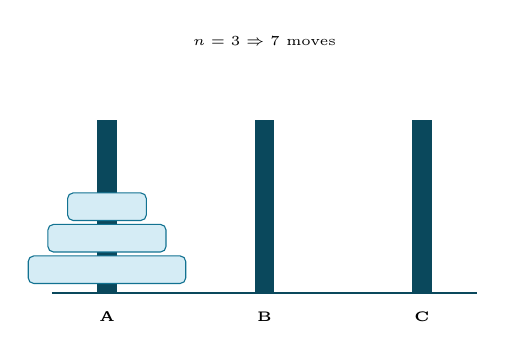
\begin{tikzpicture}[
        peg/.style={draw=PrimaryDark,fill=PrimaryDark,minimum width=0.15cm,
                    minimum height=2.5cm},
        disk/.style={draw=PrimaryMid,fill=PrimaryLight!60,rounded corners=2pt,
                     minimum height=0.35cm}
      ]
        \node[peg,minimum height=2.2cm] at (0,1.1) {};
        \node[peg,minimum height=2.2cm] at (2,1.1) {};
        \node[peg,minimum height=2.2cm] at (4,1.1) {};
        \node[disk,minimum width=2.0cm] at (0,0.3) {};
        \node[disk,minimum width=1.5cm] at (0,0.7) {};
        \node[disk,minimum width=1.0cm] at (0,1.1) {};
        \draw[PrimaryDark,thick] (-0.7,0) -- (4.7,0);
        \node[font=\tiny\bfseries] at (0,-0.3) {A};
        \node[font=\tiny\bfseries] at (2,-0.3) {B};
        \node[font=\tiny\bfseries] at (4,-0.3) {C};
        \node[font=\tiny] at (2,3.2)
          {$n=3 \Rightarrow 7$ moves};
      \end{tikzpicture}
      \vspace{0.3em}
      \begin{alertblock}{Combinatorial explosion}
        $n=64$ requires $2^{64}{-}1 \approx 1.8\times10^{19}$ moves.
        At 1 move/sec that is \textbf{584 billion years}.
      \end{alertblock}
  \end{columns}
\end{frame}

\begin{frame}[shrink=12]{Recursive Analysis: Counting Binary Digits}
  \begin{columns}[T]
    \column{0.50\textwidth}
      \begin{block}{\textsc{BinRec}$(n)$}
        \begin{algorithmic}[1]
          \Require positive integer $n$
          \Ensure \# binary digits of $n$
          \If{$n = 1$} \Return $1$ \EndIf
          \State \Return $\textsc{BinRec}(\lfloor n/2 \rfloor) + 1$
        \end{algorithmic}
      \end{block}
      \vspace{0.3em}
      \textbf{Recurrence:}
      \[
        A(n) = A\!\left(\lfloor n/2\rfloor\right) + 1, \quad A(1) = 0
      \]
    \column{0.45\textwidth}
      \textbf{Solution:} Assume $n = 2^k$:
      \begin{align*}
        A(2^k) &= A(2^{k-1}) + 1 \\
               &= A(2^{k-2}) + 2 \\
               &= \ldots = A(2^0) + k = k
      \end{align*}
      Since $k = \log_2 n$:
      \[
        \boxed{A(n) = \lfloor\log_2 n\rfloor \in \Theta(\log n)}
      \]
      \vspace{0.3em}
      Each recursion halves $n$ → depth $= \log_2 n$ levels.
  \end{columns}
\end{frame}

% ============================================================
\section{Useful Summation Formulas}
% ============================================================

\begin{frame}[shrink=28]{Essential Summations for Analysis}
  \begin{columns}[T]
    \column{0.50\textwidth}
      \textbf{Constant sum:}
      \[
        \sum_{i=a}^{b} c = c\,(b-a+1)
      \]
      \textbf{Arithmetic series:}
      \[
        \sum_{i=1}^{N} i = \frac{N(N+1)}{2} \in \Theta(N^2)
      \]
      \[
        \sum_{i=0}^{N-1} i = \frac{N^2-N}{2}
      \]
      \textbf{Quadratic series:}
      \[
        \sum_{i=1}^{N} i^2 = \frac{N(N+1)(2N+1)}{6} \in \Theta(N^3)
      \]
    \column{0.45\textwidth}
      \textbf{Geometric series:}
      \[
        \sum_{i=0}^{N} a^i = \frac{a^{N+1}-1}{a-1} \qquad (a\neq 1)
      \]
      \[
        \sum_{i=0}^{N} 2^i = 2^{N+1} - 1 \in \Theta(2^N)
      \]
      \textbf{Harmonic series:}
      \[
        \sum_{i=1}^{N} \frac{1}{i} \approx \ln N \in \Theta(\log N)
      \]
      \vspace{0.3em}
      \begin{exampleblock}{Application}
        These formulas are the core tools for converting summations
        from loop analyses into closed-form complexities.
      \end{exampleblock}
  \end{columns}
\end{frame}

% ── Chapter Summary ──────────────────────────────────────────
\begin{frame}[shrink=12]{Chapter 2 Summary}
  \begin{columns}[T]
    \column{0.50\textwidth}
      \textbf{Key concepts:}
      \begin{itemize}
        \item $T(n)\approx c_{\mathrm{op}}\cdot C(n)$: count basic operations
        \item $\mathcal{O}(f)$: upper bound; $\Omega(g)$: lower bound;
              $\Theta(h)$: tight bound
        \item Use the \emph{limit method} to establish growth order
        \item Four general rules for iterative analysis
        \item Recurrences: telescoping, Master Theorem
        \item Typical growth hierarchy:
              $\log n \ll n \ll n\log n \ll n^2 \ll 2^n \ll n!$
      \end{itemize}
    \column{0.45\textwidth}
      \begin{block}{Next chapter}
        \textbf{Chapter 3:} Brute Force \& Exhaustive Search —
        the simplest strategy: try everything.
        We analyse selection sort, bubble sort, string matching,
        and combinatorial problems.
      \end{block}
      \vspace{0.3em}
      \begin{exampleblock}{Self-check questions}
        \begin{enumerate}
          \item What is $\Theta$ for $T(n) = 5n^3 - 2n^2 + 100$?
          \item Solve: $T(n) = T(n-1) + n,\; T(1)=1$
          \item Is $n! = \mathcal{O}(n^n)$? Prove it.
        \end{enumerate}
      \end{exampleblock}
  \end{columns}
\end{frame}

\end{document}
